\documentclass[11pt,letterpaper]{article}
\usepackage{graphicx}
\usepackage{common}
\usepackage{amsmath,amsfonts,amssymb,bbm}
\usepackage{palatino}
\usepackage[linkcolor=blue]{hyperref}
\usepackage{fullpage}
\usepackage{color}
\usepackage{enumitem}
\usepackage{titlesec}
\usepackage[textsize=tiny]{todonotes}
\newcommand{\TODO}[1]{\todo[inline]{#1}}
\newcommand{\R}{\mathbbm{R}}
\newcommand{\mba}{\mathbf{a}}
\newcommand{\mbb}{\mathbf{b}}
\newcommand{\mbx}{\mathbf{x}}
\newcommand{\mbxt}{\tilde{\mathbf{x}}}
\newcommand{\Sigmat}{\tilde{\Sigma}}
\newcommand{\mbz}{\mathbf{z}}
\newcommand{\mbw}{\mathbf{w}}
\newcommand{\eps}{\epsilon}
\newcommand{\Ut}{\tilde{U}}
\newcommand{\angstrom}{\textup{\AA}}
\newcommand{\E}{\mathrm{E}}
\newcommand{\Var}{\mathrm{Var}}
\newcommand{\p}{\partial}
\renewcommand*{\thefootnote}{\fnsymbol{footnote}}

\newboolean{solutionCopy}
\setboolean{solutionCopy}{true} % Toggle between solution copy and distro

\ifthenelse{\boolean{solutionCopy}}{
  \includeversion{solution}
}{
  \excludeversion{solution}
}


\begin{document}

\ifthenelse{\boolean{solutionCopy}}{
\begin{center}
{\LARGE CS 181 Spring 2017 Section 5\\
Margin-Based Classification, SVMs\\
Solution}
\end{center}
}{
  \begin{center}
{\LARGE CS 181 Spring 2017 Section 5}\\
Margin-Based Classification, SVMs
\end{center}
}

\section{Motivation}
The idea for Support Vector Machines is that, for all the linear hyperplanes that exist, we want one that will create the largest distance, or ``margin'', with the training data. Larger margins tend to improve generalization error. To define the margin, we consider a hyperplane of the form
$$\boldw^\top \boldx + w_0 = 0$$

\noindent\fbox{\parbox{\linewidth}{%
{What is the perpendicular distance from an example $\boldx_i$ 
to the decision boundary $\boldw^\top \boldx + w_0 = 0$?}.
}}

\medskip 

\noindent For two points $\boldx_1$ and $\boldx_2$ on the hyperplane, consider the projection with $\boldw$:
$$\boldw^\top(\boldx_1 - \boldx_2) = \boldw^\top\boldx_1 - \boldw^\top\boldx_2 = -w_0 -(-w_0) = 0$$
Therefore, $\boldw$ is orthogonal to the hyperplane. So to get the distance from a hyperplane and an arbitrary example $\boldx$, we just need the length
in the direction of $\boldw$ between the point and the hyperplane. We let $r$ signify the distance between a point and the hyperplane. Then $\boldx_{\perp}$ is the projection of the point onto the hyperplane,
so that we can decompose a point $\boldx$ as
%
$$
\boldx_{\perp}+r\frac{\boldw}{||\boldw||} = \boldx
$$

\noindent Left multiply by $\bold w^\top$:
$$
\boldw^\top\boldx_{\perp} + r\frac{\boldw^\top\boldw}{||\boldw||} = \boldw^\top\boldx \Rightarrow r = \frac{\boldw^\top\boldx+w_0}{||\boldw||}
$$

\noindent Scalar $r$ then gives the signed, normalized distance between a point and the hyperplane.
For correctly classified data, we have $y_i=+1$ when this distance is
positive and $y_i=-1$ when it is negative. Based on this,
we can obtain a positive distance for both kinds of examples
by multiplying by $y_i$. We define the margin of the dataset as the minimum such
distance over all examples:
%
$$\min_{i} \frac{y_i(\boldw^\top\boldx_i + w_0)}{||\boldw||}$$

\noindent\fbox{\parbox{\linewidth}{%
{What is the training problem for support vector machines?}
}}

\medskip

\noindent We want the $\boldw$ and $w_0$ that maximize the margin:
$$\argmax_{\boldw,w_0} \frac{1}{||\boldw||} \min_i y_i(\boldw^\top\boldx_i+w_0)$$

\noindent In the hard-margin training problem, we know that the data is linearly separable and therefore any margin (including the optimal)  must be greater than 0:
%
$$
\min_{i} \frac{y_i(\boldw^\top\boldx_i + w_0)}{||\boldw||}>0
$$

\noindent We can observe that $\boldw$ and $w_0$ are invariant to changes of scale.
Because of this, it is without loss of generality to impose
$\min_{i} \frac{y_i(\boldw^\top\boldx_i + w_0)}{||\boldw||}>1$. This lets
us write the optimization problem as:
%
$$
\argmax_{\boldw, w_0} \frac{1}{||\boldw||} \quad \text{ s.t. }\forall i\text{ } y_i(\boldw^\top\boldx_i+w_0) \geq 1
$$

\noindent\fbox{\parbox{\linewidth}{%
{What is the corresponding minimization problem for
hard-margin training for SVMs?}\\\\
{Explain at a high level why the minimization problem for SVMs is equivalent to the max-margin problem.}
}}
\medskip
\noindent We can invert $\boldw$ to change the max to a min:
$$
\argmin_{\boldw, w_0} \frac{1}{2}||\boldw||^2 \quad \text{ s.t. }\forall i\text{ }
y_i(\boldw^\top\boldx_i+w_0) \geq 1$$

\noindent Informally, this is the same as max-margin training because the constraint
is binding for the examples closest to the decision boundary. For
these examples we have $y_i(\boldw^\top\boldx_i+w_0) = 1$.  The
distance on these examples is $1/||\boldw||$, and is maximized by
minimizing $||\boldw||^2$.


\section{Soft Margin Formulation}

For the hard margin formulation, we have been assuming that the data
is linearly separable. However, this is not always true, and even
if the data is linearly separable, it may not be best to find a
separating hyperplane. In optimizing generalization error, there is a
tradeoff between the size of the margin and the number of mistakes on
the training data.\\

\noindent For the soft margin formulation, we introduce a slack variable $\xi_i
\geq 0$ for each $i$ to relax the constraints on each example.
%
$$
\xi_i \begin{cases} 
      =0 & \text{if correctly classified} \\
      \in (0,1] & \text{correctly classified but inside margin
        region}\\
      >1 & \text{if incorrectly classified}
   \end{cases}
$$

\noindent We can now rewrite
the training problem
for a soft margin formulation to be 
%
$$
\argmin_{\boldw, w_0} \frac{1}{2}{||\boldw||^2} + C\sum_{i=1}^n \xi_i $$
$$\text{ s.t. }\forall i\text{ } y_i(\boldw^\top\boldx_i+w_0) \geq 1 - \xi_i$$
$$ \xi_i \geq 0$$


\noindent We add a regularization parameter $C$, that controls how much we
penalize violating the hard margin constraints. 
A large $C$ penalizes these violations and thus
``respects'' the data closely and has small regularization.  A small
$C$ does not penalize the sum of slack variables as heavily, relaxing
the constraint. This is increasing the regularization.

\section{Dual Form of the Support Vector Machine Training Problem}

\noindent\fbox{\parbox{\linewidth}{
Use Lagrange multipliers to convert the new minimization problem into dual form.
}}
\medskip

\noindent Our original hard-margin training problem, which looks for weights
that maximize the margin on the training data, is
%
\begin{align}
\label{eq:opt-problem-constraint}
\boldw^\star, w_0^\star &=
\argmin_{\boldw,w_0}\ \frac{1}{2}||\boldw||^2 \quad \mbox{s.t.}
\quad y_i(\boldw^\top\boldx_i+w_0)\geq 1, \quad \forall i\in
\{1,\ldots,n\}\,.
\end{align}

\noindent We introduce {\em Lagrange multipliers},~${\alpha_1, \ldots, \alpha_n \geq 0}$, 
one for each inequality in Equation~\ref{eq:opt-problem-constraint}, i.e., one per example, to obtain the Lagrangian function (Bishop appendix E does a good job of explaining Lagrange multipliers):
\begin{align}
L(\boldw,w_0,\balpha) &= \frac{1}{2}||\boldw||^2
-\sum_{i=1}^n\alpha_i(y_i(\boldw^\top\boldx_i+w_0)-1)\,
\end{align}

\noindent Based on this, we now equivalently solve:
%
$$
\boldw^*, w_0^* = \argmin_{\boldw,w_0} \max_{\boldsymbol{\alpha} \geq 0}L(\boldw, w_0, \balpha)
$$

\noindent By strong duality (out of scope!),
we can  equivalently write this as:
%
$$\max_{\boldsymbol{\alpha} \geq 0}\min_{\boldw,w_0} L(\boldw,w_0,\balpha)$$

\noindent This is useful because we can now solve
analytically for the $\min_{\boldw,w_0}[\cdot]$
part of this expression. Taking derivatives, we see:
%
$$\frac{\partial L}{\partial w_j} = w_j - \sum_{i=1}^n \alpha_iy_i\boldx_i = 0 \Rightarrow \boldw^* = \sum_{i=1}^n \alpha_iy_i\boldx_i$$
$$\frac{\partial L}{\partial w_0} = -\sum_{i=1}^n \alpha_iy_i = 0 \Rightarrow \sum_{i=1}^n \alpha_iy_i = 0$$

\noindent Plugging these optimal values into the Lagrangian function, we get
(you should understand but not memorize this):
%
\begin{align*}
L(\boldw, w_0, \balpha) &= \frac{1}{2}||\sum_{i=1}^n \alpha_iy_i\boldx_i||^2 - \sum_{i=1}^n \alpha_iy_i(\sum_{i'=1}^n \alpha_{i'}y_{i'}\boldx_{i'})^\top\boldx_i
- \sum_{i=1}^n\alpha_iy_iw_0 + \sum_{i=1}^n \alpha_i \\
&= \frac{1}{2} \sum_{i=1}^n \sum_{i'=1}^n \alpha_i \alpha_{i'} y_i y_{i'} \boldx_i^\top \boldx_{i'} - \sum_{i=1}^n \sum_{i'=1}^n \alpha_i \alpha_{i'} y_i y_{i'} \boldx_i^\top \boldx_{i'} - w_0 \sum_{i=1}^n \alpha_i y_i + \sum_{i=1}^n \alpha_i \\
&= \sum_{i=1}^n \alpha_i - \frac{1}{2}\sum_{i=1}^n \sum_{i'=1}^n \alpha_i\alpha_{i'}y_iy_{i'} \boldx_i^\top \boldx_{i'}
\end{align*}

\noindent We then solve for $\balpha$, maximizing $L$,
subject to $\balpha\geq 0$. The support
vectors are defined to be $Q = \{i : \alpha_i > 0\}$.
For the soft-margin variation, these include examples
that lie in the margin region in addition
to on the margin boundary.
	
\section{Why bother with the dual form? *very important*}

\noindent The dual form is useful because the number of variables to maximize
is linear in $n$ (one for each training example), and does not depend on
the dimension of the feature space! Moreover, there tends to
be a small number of support vectors (data points that define the boundary)
and thus the trained classifier can be interpretable. \\

\noindent To classify a new example $\boldx$, we compute 

$$\sum_{i=1}^n\alpha^\star_i \,y_i \boldx_i^\top \boldx+w_0^\star$$

\noindent where $\alpha^\star$ and $w_0^\star$ solve
the training problem. Based on this, we classify the example
as $+1$ if this discriminant value is $>0$, and $-1$ otherwise. 

\noindent In addition, the dual has the very nice property that 
if we use a basis function to map $\boldx$ to a higher dimensional space, 
this only comes in through the ``kernel function.''
The training problem is as explained earlier, except where
$\boldx_i^\top \boldx_{i'}$ appears, we use 
%
\begin{align*}
K(\boldx_i,\boldx_{i'})&=\bphi(\boldx_i)^\top\bphi(\boldx_{i'})
\end{align*}

\noindent in its place. Similarly, we classify  a new example $\boldx$
based on the value of discriminant 
$\sum_{i=1}^n\alpha^\star_i \,y_i K(\boldx_i,\boldx)
+w_0^\star$. The reason that this is interesting
is because we can directly compute the dot product
$\bphi(\boldx)^\top \bphi(\boldx')$
{\em without projecting to the higher-dimensional space!}
This is known as the ``kernel trick.''
As long as $K()$ is a valid kernel (see practice question below)
the dual training problem can be solved without actually computing $\bphi$.

\newpage
\section{Practice Problems (cover some but not all at section)}
\begin{enumerate}

\item {\bf Removing Support Vectors and Retraining (Berkeley, Fall '11)}\\
\fbox{\parbox{\linewidth}{%
    Suppose that we train two SVMs, the first containing all of the
    training data and the second trained on a data set constructed by 
    removing some of the support vectors from the first training set. 
    How does the size of the optimal margin change between the first and second training data?
    What is a downside to doing this?

}}

\begin{solution}
\vspace{\baselineskip}
If we remove some of the examples on the margin
(the examples that are closest to the best separator), then we can
either leave the size of the optimal margin the same or we can
increase the size of the optimal margin. 
This is because we have removed the difficult examples, and thus we can either
leave the optimal solution unchanged or make it ``better" (corresponding to increasing 
the size of the optimal margin). A potential downside is that we might see
equally difficult points at test time and mis-classify them.
\vspace{\baselineskip}

\end{solution}

\ifthenelse{\boolean{solutionCopy}}{}{
  \vspace{4cm}
}

\item {\bf Proof that margin is invariant to scalar 
multiplication}\\
\fbox{\parbox{\linewidth}{%
    In reformulating our max margin $$\frac{y_i(\boldw^\top \boldx_i+w_0)}{|| \boldw ||}$$ training problem, we use the fact that the
    margin is invariant to multiplying $(\boldw, w_0)$ by any $\beta > 0$. Show that this property is true.
}}

\begin{solution}

\vspace{\baselineskip}

$$
 \frac{y_i((\beta\boldw)^\top \boldx_i + (\beta w_0))}{|| (\beta \boldw) ||}= \frac{\beta}{\beta} \cdot \frac{y_i(\boldw^\top \boldx_i+w_0)}{|| \boldw ||}   =\frac{y_i(\boldw^\top \boldx_i+w_0)}{|| \boldw ||} $$

\vspace{\baselineskip}

\end{solution}


\ifthenelse{\boolean{solutionCopy}}{}{
  \vspace{4cm}
}

\item {\bf  (Berkeley, Fall '11)}

\fbox{\parbox{\linewidth}{%
    Consider $\boldx,\boldx'\in\mathbb{R}^2$.
    Show that the polynomial kernel of degree 2, $K(\boldx, \boldx' ) = (1 + \boldx^\top \boldx')^2$ is equivalent to
    a dot product $\boldsymbol{\phi}(\mathbf{x})^\top\boldsymbol{\phi}(\mathbf{x^\prime})$ where 
    $\boldsymbol{\phi}(\mathbf{x})=(x_1^2, x_2^2, x_1, x_2, x_1x_2,1)$.
}}

\begin{solution}

\vspace{\baselineskip}

The dot product of the features $\bphi(\boldx)$ and $\bphi(\boldx')$ is 
$x_1^2 {x'_1}^2 + x_2^2 {x'_2}^2 + x_1 x'_1 + x_2 x'_2 + x_1x_2 x'_1 x'_2 + 1$. 
The kernel function gives:
\begin{align*}
K(\boldx, \boldx') &= (1 + \boldx^\top \boldx')^2 \\
&= (1 + x_1x'_1 + x_2x'_2)^2\\
&= 1 + 2x_1x'_1 + 2x_2x'_2 + 2x_1x'_1x_2x'_2 + x_1^2{x'_1}^2 + x_2^2{x'_2}^2
\end{align*}
So the dot product and kernel function give the same terms (up to scalar
multiples in terms),  meaning they are equivalent.

\vspace{\baselineskip}

\end{solution}

\newpage

\item {\bf Composing Kernels}

\fbox{\parbox{\linewidth}{%


  \noindent A key benefit of SVM training is the ability to use kernel functions
  $K(\boldx, \boldx')$ as opposed to explicit basis functions
  $\bphi(\boldx)$. Kernels make it possible to implicitly express
  large or even infinite dimensional basis features. We do this 
  by computing $\bphi(\boldx)^\top\bphi(\boldx')$ directly, without 
  ever computing $\bphi(\boldx)$.\\

  \noindent When training SVMs, we begin by computing the kernel matrix $\boldK$,
  over our training data $\{\boldx_1, \ldots, \boldx_n\}$.  The kernel
  matrix, defined as $K_{i, i'} = K(\boldx_i, \boldx_{i'})$, expresses
  the kernel function applied between all pairs of training points.\\

  \noindent In class, we saw Mercer's theorem (maybe), which tells us that any function
  $K$ that yields a positive semi-definite kernel matrix forms a valid
  kernel, i.e. corresponds to a matrix of dot-products under
  \textit{some} basis $\bphi$. Therefore instead of using an explicit
  basis, we can build kernel functions directly that fulfill this
  property.\\

  \noindent A particularly nice coralary of this theorem is that it allows us to
  build more expressive kernels by composition.  In this problem, you
  are tasked with using Mercer's theorem and the definition of a
  kernel matrix to prove that the following  compositions are valid kernels, 
  assuming $K^{(1)}$ and $K^{(2)}$ are valid kernels. Recall that a positive semi-definite matrix $\boldK$ requires $\mathbf{z}^\top \mathbf{Kz} \geq 0,\ \forall\ \mathbf{z} \in \reals^n$.

  \begin{enumerate}
  \item $K(\boldx, \boldx') = c\,K^{(1)}(\boldx, \boldx') \quad \text{for $c>0$}$
  \item $   K(\boldx, \boldx')= K^{(1)}(\boldx, \boldx') + K^{(2)}(\boldx, \boldx')$
  \item   $ K(\boldx, \boldx') = f(\boldx)\,K^{(1)}(\boldx, \boldx')\,f(\boldx') \quad
  \text{where $f$ is any function from~$\reals^m$ to $\reals$}$
  \item $ K(\boldx, \boldx') = K^{(1)}(\boldx, \boldx')\,K^{(2)}(\boldx,
  \boldx')$

  [Hint: Use the property that for any
  $\bphi(\boldx)$,
  $K(\boldx, \boldx') = \bphi(\boldx)^\top\bphi(\boldx')$ forms a
  positive semi-definite kernel matrix. ]
  \item 
  \begin{enumerate}
    \item The $\exp$ function can be written as,
    $$\exp(x) = \lim_{i\rightarrow \infty} \left(1 + x + \cdots + \frac{x^i}{i!}\right).$$
      Use this to show that $\exp(xx')$ (here
          $x, x'\in \reals$)) can be written as $\bphi(x)^\top \bphi(x')$ for some basis function $\bphi(x)$. Derive this basis function,
          and explain why this  would be hard to use as a basis in standard logistic regression.
    \item Using the previous identities, show that $K(\boldx, \boldx') = \exp( K^{(1)}(\boldx, \boldx'))$ is a valid kernel.
  \end{enumerate}
  \item  Finally use this analysis and previous identities to prove the validity of the Gaussian kernel:
  \begin{align*}
  K(\boldx, \boldx') &= \exp \left( \frac{-||\boldx - \boldx'||^2_2}{2\sigma^2} \right) 
  \end{align*}
  \end{enumerate}
}}

\newpage

\begin{solution}

\vspace{\baselineskip}


    \noindent For parts 1-5, it suffices to show that the kernel is valid either by 
    finding a particular $\bphi(\boldx)$ that produces it, or by showing that the kernel matrix 
    is positive semi-definite. In these solutions, let $\bphi^{(i)}(\boldx)$ and $\mathbf{K}^{(i)}$ 
    denote the underlying basis function and kernel matrix for kernel $K^{(i)}$, respectively.
    \begin{enumerate}
      \item We have the kernel matrix $\mathbf{K} = c \mathbf{K}^{(1)}$. We need $\mathbf{v}^\top \mathbf{K} \mathbf{v} = c \mathbf{v}^\top \mathbf{K}^{(1)} \mathbf{v} \geq 0$, which we know to be true because $\mathbf{K}^{(1)}$ is positive semi-definite and $c > 0$.\\
      Alternatively, take $\bphi(\boldx) = \sqrt{c} \; \bphi^{(1)}(\boldx)$.

      \item We have the kernel matrix $\mathbf{K} = \mathbf{K}^{(1)} + \mathbf{K}^{(2)}$. We need 
      $$\mathbf{v}^\top \mathbf{K} \mathbf{v} = \mathbf{v}^\top(\mathbf{K}^{(1)} + \mathbf{K}^{(2)})\mathbf{v} = \mathbf{v}^\top\mathbf{K}^{(1)}\mathbf{v} + \mathbf{v}^\top\mathbf{K}^{(2)}\mathbf{v} \geq 0,$$
      which we know to be true because $\mathbf{K}^{(1)}, \mathbf{K}^{(2)}$ are positive semi-definite.\\
      Alternatively, take $\bphi(\boldx) = \left[\phi_1^{(1)}(\boldx), \hdots, \phi_d^{(1)}(\boldx), \phi_1^{(2)}(\boldx), \hdots, \phi_d^{(2)}(\boldx)\right]^\top$, the concatenation of $\bphi^{(1)}(\boldx), \bphi^{(2)}(\boldx)$

      \item Take $\bphi(\boldx) = f(\boldx)\bphi^{(1)}(\boldx)$.

      \item Take $\bphi(\boldx) = \left[\phi_1^{(1)}(\boldx)\phi_1^{(2)}(\boldx), \hdots, \phi_1^{(1)}(\boldx)\phi_d^{(2)}(\boldx), \phi_2^{(1)}(\boldx)\phi_1^{(2)}(\boldx), \hdots, \phi_d^{(1)}(\boldx)\phi_d^{(2)}(\boldx) \right]^\top$, the flattened vector for outer product $\bphi^{(1)}(\boldx) \otimes \bphi^{(2)}(\boldx)$. The order of terms does not matter.

      \item \begin{enumerate}
        \item Using the Taylor series expansion, we see that $\exp(xx') = \lim_{i\rightarrow \infty} \left(1 + xx' + \cdots + \frac{(xx')^i}{i!}\right)$. Take 
        $$\bphi(x) = \left[1, x, \hdots, \frac{x^i}{\sqrt{i!}}, \hdots \right]^\top.$$
        This is infeasible because we have an infinite basis!

        Note: don't forget the square root on the factorial in the denominator.
        \item We have
        $$K(\boldx, \boldx') = \exp\left( K^{(1)}(\boldx, \boldx') \right) = \exp\left(\bphi^{(1)}(\boldx)^\top \bphi^{(1)}(\boldx')\right) = \prod_{i=1}^d \exp\left(\phi_i^{(1)}(\boldx) \phi_i^{(1)}(\boldx')\right)$$
        From here, we recognize the multiplicand to be a valid kernel, using our result from part (a). Then, recognize that a product of valid kernels is a valid kernel, per our results in part 4. Alternatively, write
        $$K(\boldx, \boldx') = \exp(K^{(1)}(\boldx, \boldx')) = \lim_{i\rightarrow \infty} \left(1 + \bphi^{(1)}(\boldx)^\top\bphi^{(1)}(\boldx') + \cdots + \frac{(\bphi^{(1)}(\boldx)^\top\bphi^{(1)}(\boldx'))^i}{i!}\right)$$
        and use properties 1, 2, and 4 to recognize that this is a valid kernel.
      \end{enumerate}

      \item \begin{itemize}
        \item $K_{0}(\boldx, \boldx') = \boldx^\top\boldx'$ is a valid kernel by
          definition of the kernel (it is the inner product of $\boldx$ and
          $\boldx'$).
        \item Thus $K_{1}(\boldx, \boldx') = \exp(2\boldx^\top\boldx')$ is also a valid
          kernel by property 1 and 5.
        \item Note that $K(\boldx, \boldx') =
          \exp(-\boldx^\top\boldx)\exp(2\boldx^\top\boldx')\exp(-\boldx'^\top\boldx')
          =f(\boldx)K_{1}f(\boldx')$,
        where $f(\boldx) = \exp(-\boldx^\top\boldx)$.
        \item Hence using property 3 in the last step, we proved $K(\boldx, \boldx')$
          is a kernel.
      \end{itemize}
      Note: a common mistake is saying $\exp(-\boldx^\top\boldx)$ is a kernel.  It is
      not.

    \end{enumerate}

\vspace{\baselineskip}

\end{solution}

\newpage

\item {\bf Draw Margin Boundary}\\
\fbox{\parbox{\linewidth}{%
    In the figures below, the red examples represent
   the support vectors. All other examples can be assumed to have $\alpha_i = 0$. Draw the margins for the boundary given this information.
   \\
   i) For the first example, you can assume the hard margin formulation. Draw the decision boundary as well as the two margin boundaries given the support vector.
   \\
   ii) For the second example, you can assume the soft margin formulation and that all points are correctly classified with the optimal decision boundary. The decision boundary is already given. Draw the two margin boundaries given the support vector.
}}
\\
\\
\\
i)
\begin{center}
 \begin{tikzpicture}[x=1cm,y=.6cm]


 \draw[latex-latex, thin, draw=gray] (-4,0)--(4,0) node [right] {$x_1$}; % l'axe des abscisses
 \draw[latex-latex, thin, draw=gray] (0,-5)--(0,5) node [above] {$x_2$}; % l'axe des ordonnées



\foreach \Point in {(-2,1.5), (-1,1),(1,1), (-2,3), (-1,2.5), (1,3),(2,4), (2,3)}{
    \node[color=red] at \Point {\textbullet};
}
\foreach \Point in {(-2,1.5), (-1,1), (-2,3), (-1,2.5), (1,3),(2,4), (2,3)}{
    \node at \Point {\textbullet};
}


\foreach \Point in {(2,-1.5), (1,-1), (2,-3), (1,-2.5), (1,-3), (3,-2), (3,0), (3,1), (1,.2)}{
    \node at \Point {$\circ$};
}

% to ensure that the points are being properly centered:
\draw [dotted, gray] (-4,-6) grid (5,5);
\node [color=red,label={[shift={(.5,-1)}]}] at (1,.2) {$\circ$};
\node [color=red,label={[shift={(.6,-.8)}]}] at (1,1) {$\circ$};
\node [color=red,label={[shift={(.5,0)}]}] at (3,1) {$\circ$};

\end{tikzpicture}
\end{center}

ii)
\begin{center}
 \begin{tikzpicture}[x=1cm,y=.6cm]


 \draw[latex-latex, thin, draw=gray] (-4,0)--(4,0) node [right] {$x_1$}; % l'axe des abscisses
 \draw[latex-latex, thin, draw=gray] (0,-5)--(0,5) node [above] {$x_2$}; % l'axe des ordonnées
%  \draw[thick] (-3,-2)--(3,4); % l'axe des abscisses

\foreach \Point in {(-2,1.5), (-1,1), (-2,3), (-1,2.5), (1,3),(2,4),(1,1), (2,3)}{
    \node[color=red] at \Point {\textbullet};
}

\foreach \Point in {(-2,1.5), (-1,1), (-2,3), (-1,2.5), (1,3),(2,4)}{
    \node at \Point {\textbullet};
}

\foreach \Point in {(2,-1.5),  (2,-3), (1,-2.5), (1,-3), (3,-2), (3,0), (3,1), (1,.2)}{
    \node at \Point {$\circ$};
}

% to ensure that the points are being properly centered:
\draw [dotted, gray] (-4,-6) grid (5,5);
 \draw[latex-latex, thin, draw=gray] (-4,-4.5)--(4,3.5) node [above] {$x_2$}; % l'axe des ordonnées

\node [color=red,label={[shift={(0,-1)}]\tiny{$\xi > 0$}}] at (1,.2) {$\circ$};
\node [color = red,label={[shift={(0,-1)}]\tiny{$\xi > 0$}}] at (1,1) {$\circ$};
\node [color=red,label={[shift={(0,-1)}]\tiny{$\xi = 0$}}] at (2,3) {$\circ$};

\node [color=red,label={[shift={(0,-1)}]\tiny{$\xi=0$}}] at (3,1) {$\circ$};

\end{tikzpicture}

\end{center}

\begin{solution}

\vspace{\baselineskip}

i)
\begin{center}
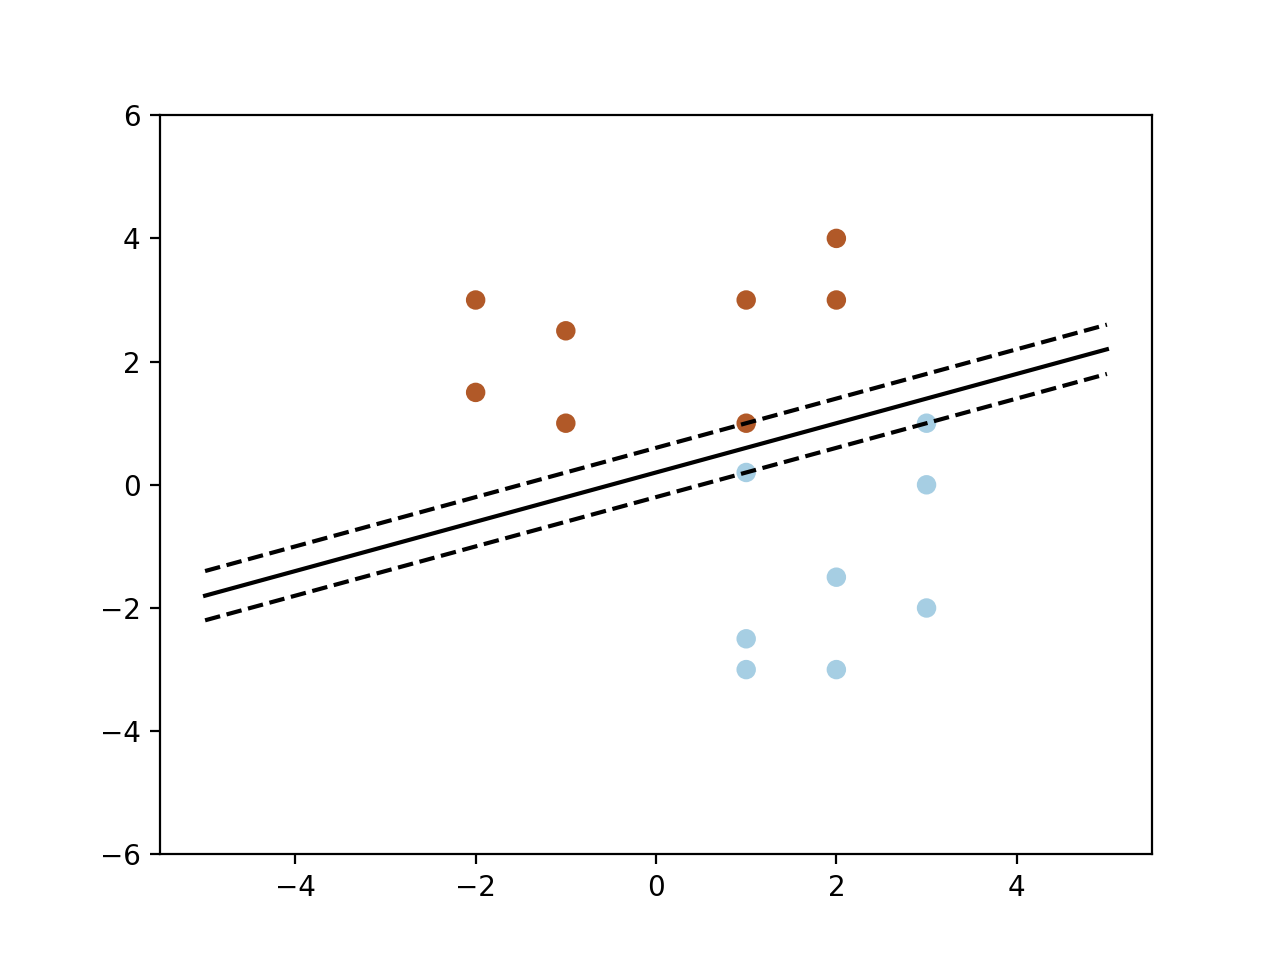
\includegraphics[scale = .8]{hard_margin.png}
\end{center}
ii)
\begin{center}
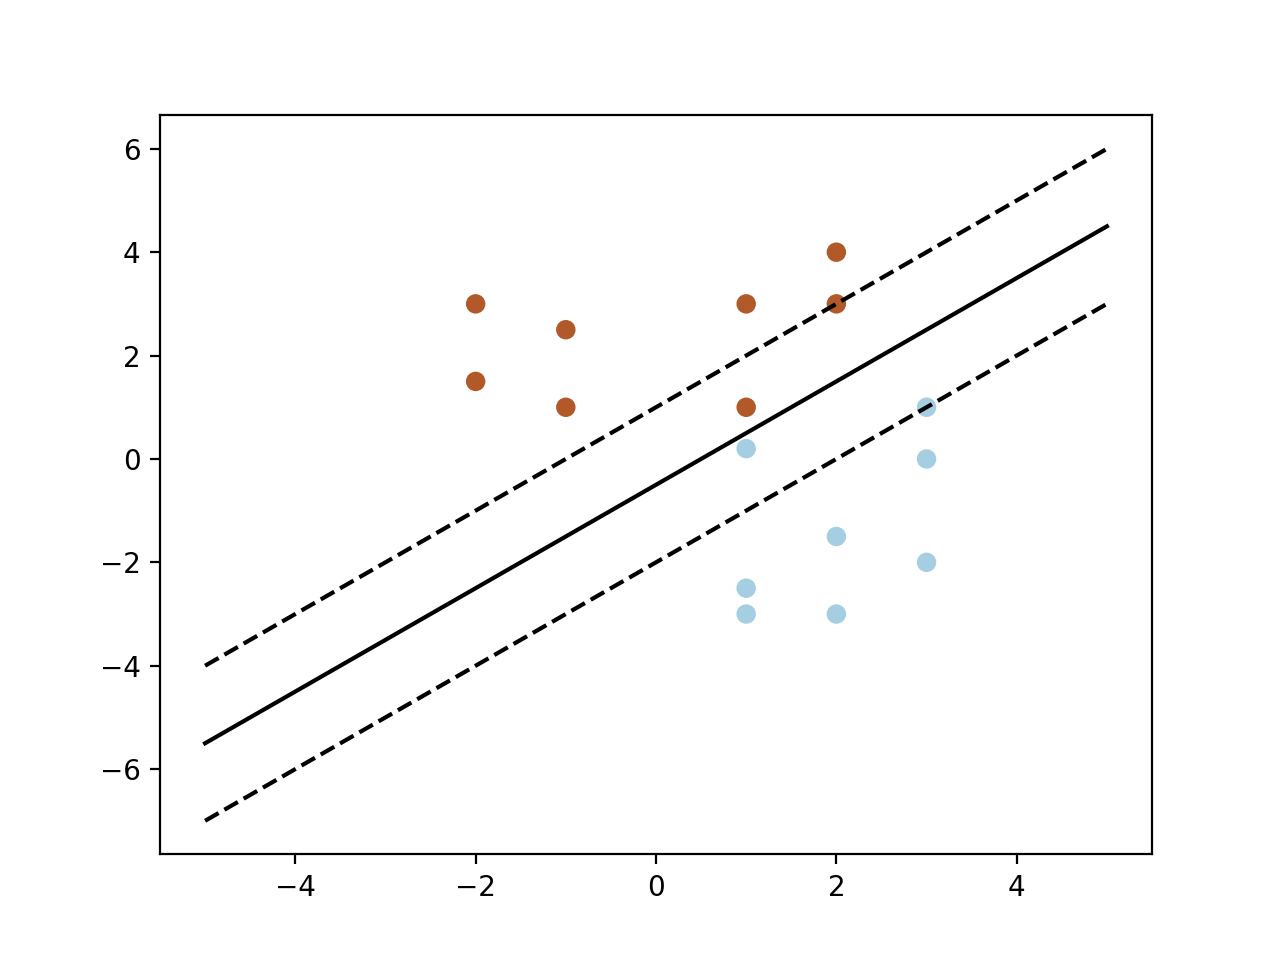
\includegraphics[scale = .8]{soft_margin.png}
\end{center}

\vspace{\baselineskip}

\end{solution}


%The more points we allocate
%with $\alpha_i > 0$, the larger our margin boundary grows as you soften the co%nstraints. 

  
\newpage

\vspace{1cm}

\item {\bf  String Kernel}

\fbox{\parbox{\linewidth}{%
Let $\mathbf{s}$ and $\mathbf{s}'$ be strings. To measure how similar $\mathbf{s}$ and $\mathbf{s}'$ are, consider the ``string kernel'' $K(\mathbf{s},\mathbf{s}')$, which returns the total number of distinct substrings (of any length) that $\mathbf{s}$ and $\mathbf{s}'$ have in common. For example, $K(\texttt{'aa'},\texttt{'aab'}) = 3$ because the substrings $\texttt{''}$, $\texttt{'a'}$, and $\texttt{'aa'}$ are in common.

(i) Compute $K(\texttt{'aza'},\texttt{'zaz'})$.

(ii) What is the number of possible substrings of length 1, 2, and 3
in strings that are composed from a 26-letter alphabet?

(iii) Suppose we wanted to project a string into a higher-dimensional
space such that we could represent via a 0 or 1 each of all possible
substrings of length $\leq 3$. How many dimensions would we need?

}}

\begin{solution}

\vspace{\baselineskip}

(i) $K(\texttt{'aza'},\texttt{'zaz'}) = 5$ because substrings $\texttt{''}, \texttt{'a'}, \texttt{'z'}, \texttt{'az'}, \texttt{'za'}$ are in common.

(ii) There are $26^1 = 26$ possible substrings of length 1, $26^2 = 676$ of length 2, and $26^3 = 17576$ of length 3.

(iii) Then $26 + 676 + 17576 = 18278$ features are required to represent all substrings of length $\leq 3$.

Note that in computing the kernel, we don't have to compute a feature
representation for the data points (i.e. we don't have to find the presence/absence 
of each possible substring for $\mathbf{s}$ and $\mathbf{s^\prime}$). 
Instead we can just write a program to find only the substrings that are in common. 
We avoid having to use costly representations to calculate the similarity between strings. 
This is the advantage of using kernel functions.
\vspace{\baselineskip}

\end{solution}


\end{enumerate}



\end{document}
